% from the submitted version (lines 697-737), revised
%-----------------------------------------------------------------------------------------------------
\label{sec:campus}
To test transfer to a new domain we analysed two $\sim$200\,s, 1080p phone videos of a university campus. Nothing
here needs real time, so the teacher detector YOLO26x at 1280\,px is used with BoT-SORT (ReID and motion
compensation); broken tracks are re-joined offline when motion, box size, colours and predicted attributes agree.
Two attribute heads (uniform vs.\ non-uniform, gender) are logistic-regression probes on DINOv2 features of the
RF-DETR-L backbone plus colour histograms, trained on 200 hand-labelled tracks and evaluated on 100 disjoint
random tracks; they abstain when the mean probability is within 0.35--0.65. Table~\ref{tab:campus} and
Fig.~\ref{fig:campus} summarise the outputs. Held out per person, the probes reach \PrUniAcc{}
\ci{\PrUniLo}{\PrUniHi} accuracy for dress (\PrUniCorrect/\PrUniAnswered, coverage \PrUniCov) and \PrGenAcc{}
\ci{\PrGenLo}{\PrGenHi} for gender (\PrGenCorrect/\PrGenAnswered, coverage \PrGenCov). The hand labels were
produced by the authors' AI assistant from the crops, not by independent annotators, and gender is predicted from
appearance (the uniform is gendered); it is reported only as an aggregate.

\begin{table}[!htbp]
\centering
\caption{Campus case study (YOLO26x + BoT-SORT + stitching; attributes over people with a usable crop).}
\label{tab:campus}
\footnotesize
\setlength{\tabcolsep}{2.4pt}
\begin{tabular}{lcc}
\toprule
 & video 1 & video 2 \\
\midrule
Track IDs $\rightarrow$ kept $\rightarrow$ people & \CpOneRaw{} $\rightarrow$ \CpOneKept{} $\rightarrow$ \CpOnePeople & \CpTwoRaw{} $\rightarrow$ \CpTwoKept{} $\rightarrow$ \CpTwoPeople \\
In frame, mean / peak & \CpOneMean{} / \CpOnePeak & \CpTwoMean{} / \CpTwoPeak \\
Crossings (R$\rightarrow$L/L$\rightarrow$R) & \CpOneCross{} (\CpOneCrossRl/\CpOneCrossLr) & \CpTwoCross{} (\CpTwoCrossRl/\CpTwoCrossLr) \\
Median time in view (s) & \CpOneDwell & \CpTwoDwell \\
Gender m / f / unsure & \CpOneMale{} / \CpOneFemale{} / \CpOneGUnsure & \CpTwoMale{} / \CpTwoFemale{} / \CpTwoGUnsure \\
Dress unif. / non-u. / unsure & \CpOneUniform{} / \CpOneNonUniform{} / \CpOneDUnsure & \CpTwoUniform{} / \CpTwoNonUniform{} / \CpTwoDUnsure \\
\bottomrule
\end{tabular}
\end{table}

\begin{figure}[!htbp]
\centering
\figif{fig_campus.pdf}{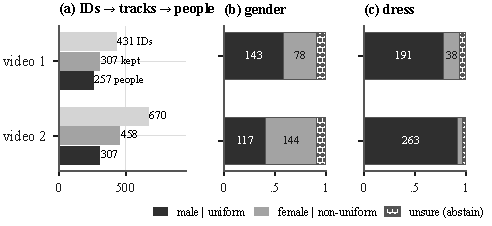
\includegraphics[width=\columnwidth]{figures/fig_campus.pdf}}
\caption{Campus case study: (a) counting funnel from raw track IDs to stitched people; (b, c) attribute shares.}
\label{fig:campus}
\end{figure}
